\section{Particle composition and detector response of hadronic recoil}
\label{app:jetcomp}

This section examines the particle composition and the detector response of the leading jet that balance the $Z$~boson in the fiducial region of the analysis.
The \powpyt{} $Z\to \mu\mu$ sample is used. The particle origin of each track is obtained using the \texttt{truthParticleLink} to find the truth identification of each reconstructed track (see section~\ref{sec:samples}). In addition to the standard event preselection described in section~\ref{sec:selection}, extra cuts are used to make sure the leading reconstructed jet matches the leading particle jet in each event.
%To ensure the closet matching between the leading reconstructed jet and leading truth jet, and always have very good DR between them, the cut on ratio of
This is achieved by requiring $|y_\mathrm{j1}|<2.1$ and $\pTlj / \pTsj < 0.7$. The selection is applied on reconstructed level. However, due to the additional criterion, the leading particle-level (truth) jet will always match the leading reco jet. Note that the jets will have a very high \pt{} since the event selection includes the selection $\pTll > \SI{165}{\GeV}$, and the jet will have a similar \pt{} to that of the $Z$~boson.


%%%%%%%%%%%%%%%%%%%%
%
% 1. TRUTH PARTICLE COMPOSITION
%


Particles are classified depending to their type in the following categories: \texttt{pion} for $\pi^+$ and $\pi^-$; \texttt{kaon} for charged kaons; \texttt{proton};
\texttt{mu} for $\mu^-$ or $\mu^+$; \texttt{e} for $e^-$ or $e^+$;
\texttt{strange} for any charge hadron with strange content other than kaons; \texttt{neutral} for any neutral hadron; \texttt{gam} for photons. 

Figure~\ref{fig:truthJetComp} presents the truth particle composition of the leading particle level jet, both in terms of multiplicity and fraction of \pt{} carried.
For the multiplicity plot, the number of photons inside the jet has been halved, since most photons originate from $\pi^0\to\gamma\gamma$, and carry less \pt{} (about half) than the other particles (hadrons) that are produced directly in the hadronization. We can see that about 44\% of the jet \pt{} is carried by charged pions, about 27\% is carried by photons and about 17\% by neutral hadrons (neutrons, $K_L$, etc.).
Figure~\ref{fig:truthChargedJetComp} presents the same two plots, but only considering charged particles. We now see that 80\% of the charged particles are pions, and they carry about 75\% of the \pt{}, indicating the average \pt{} of the charged pions inside the jet is slightly lower than that of protons and charged kaons.

\begin{figure}[b]
\centering
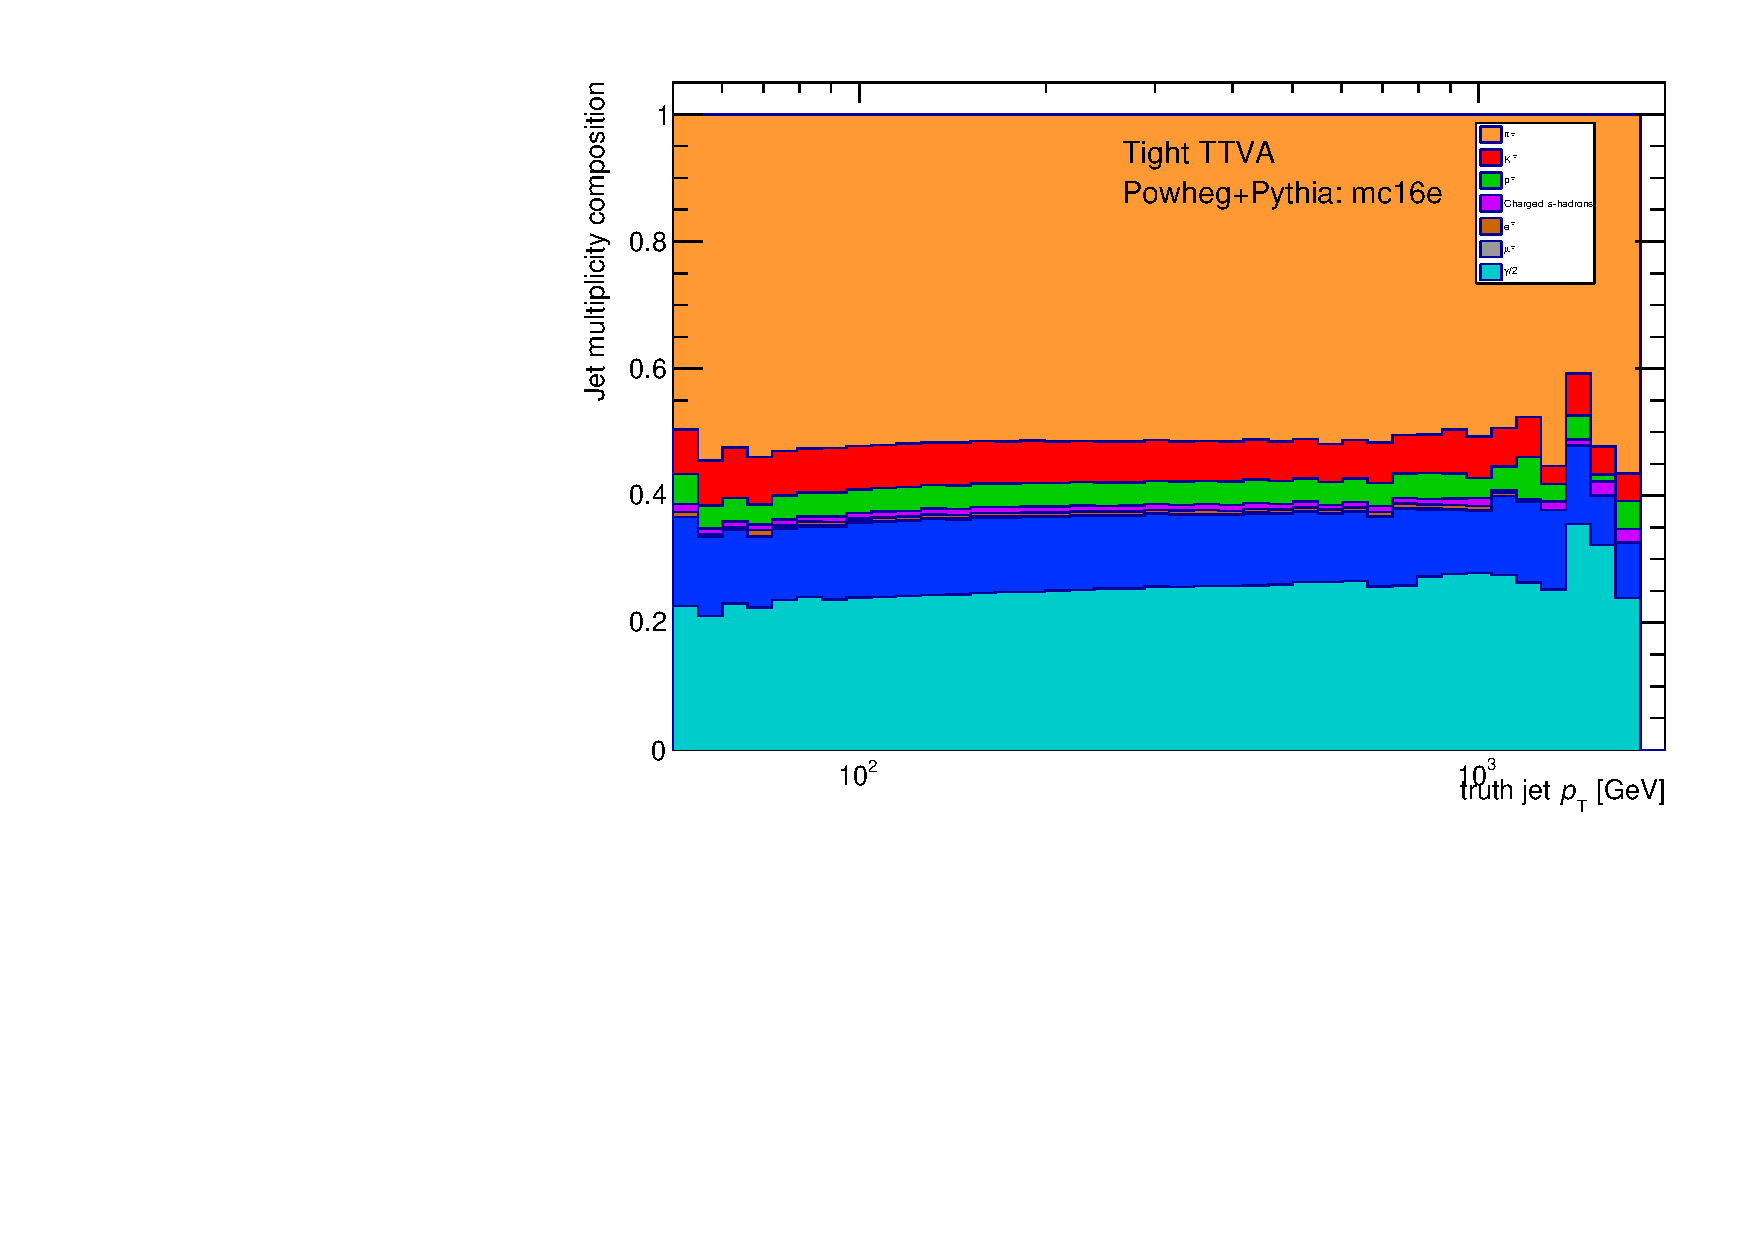
\includegraphics[width=0.48\textwidth,page=1]{figures/jet_comp_study_fixedGamma.pdf}
\includegraphics[width=0.48\textwidth,page=2]{figures/jet_comp_study_fixedGamma.pdf}%
\caption{Composition of the leading jet in terms of particle multiplicity (left) and \pt{} (right) as a function of jet \pt{}. The photon multiplicity is divided by 2 in the left plot, since most photons are produced in pairs by a neutral hadron (e.g.\ $\pi\to\gamma\gamma$).
We can see that $\approx 42$\% of the jet \pt{} is carried by neutral particles (blue, missing in legend).}
\label{fig:truthJetComp}
\end{figure}

\begin{figure}[tb]
\centering
\includegraphics[scale=0.38, page=2]{figures/jetcompstudy_MultiplicityFraction.pdf}
\includegraphics[scale=0.38, page=2]{figures/jet_comp_study_powheg_Tight_pTFraction_mc16e.pdf}%
\caption {The charged particle composition of the leading truth jet in \powpyt{} $Z$+jets MC in terms of multiplicity (left) and \pT{} (right) as a function of jet \pt{}.}
\label{fig:truthChargedJetComp}
\end{figure}


%%%%%%%%%%%%%%%%%%%%
%
% 2. Response and fake rate
%



The reconstructed tracks are required to pass track-to-vertex association (TTVA) criteria (see section~\ref{subsubsec:trigger}). 
There are three supported TTVA working points, and the studies presented below investigates two of them, namely \texttt{loose} and \texttt{tight TTVA} selection.
A looser selection means higher efficiency to reconstruct tracks matching to the desired truth particles, but also higher fraction of undesired tracks due to fake tracks, tracks from pileup particles or from secondaries.
Each reconstructed track is assigned a particle-origin label using the \texttt{truthParticleLink} associated to each track. 
The particle categories are the same as for truth particles described above.
In case there is no truth particle match to a given track, it is labelled \texttt{unmatched}. 
This category includes contributions from pileup particles and fake tracks (and possibly secondaries).


All of the tracks associated to the leading reconstructed jet are used in the study. And this jet is uniquely matched to the leading truth jet: there is always a one-to-one matching between reco $j1$ and truth $j1$.
Two quantities are studied: 
\begin{itemize}
\item
  The reconstructed track \textbf{composition} is defined as the fraction of tracks of a given category. The \textbf{multiplicity composition} is the number of tracks belonging to a given category over the total number of tracks (associated to the leading reco jet). The \textbf{$\boldsymbol{{p}_\mathrm{T}}$ composition} is the \pt{} carried by tracks of a given particle category over the total \pt{} of all tracks associated to the jet.
\item
  The pt{} \textbf{response} for a given particle type is the ratio of the \pt{} carried by tracks associated particle type over the \pt{} carried by all such truth particle. This quantity will be driven by the efficiency to reconstruct the tracks from the particle type under investigation.
\end{itemize}

\begin{figure}[b]
\centering
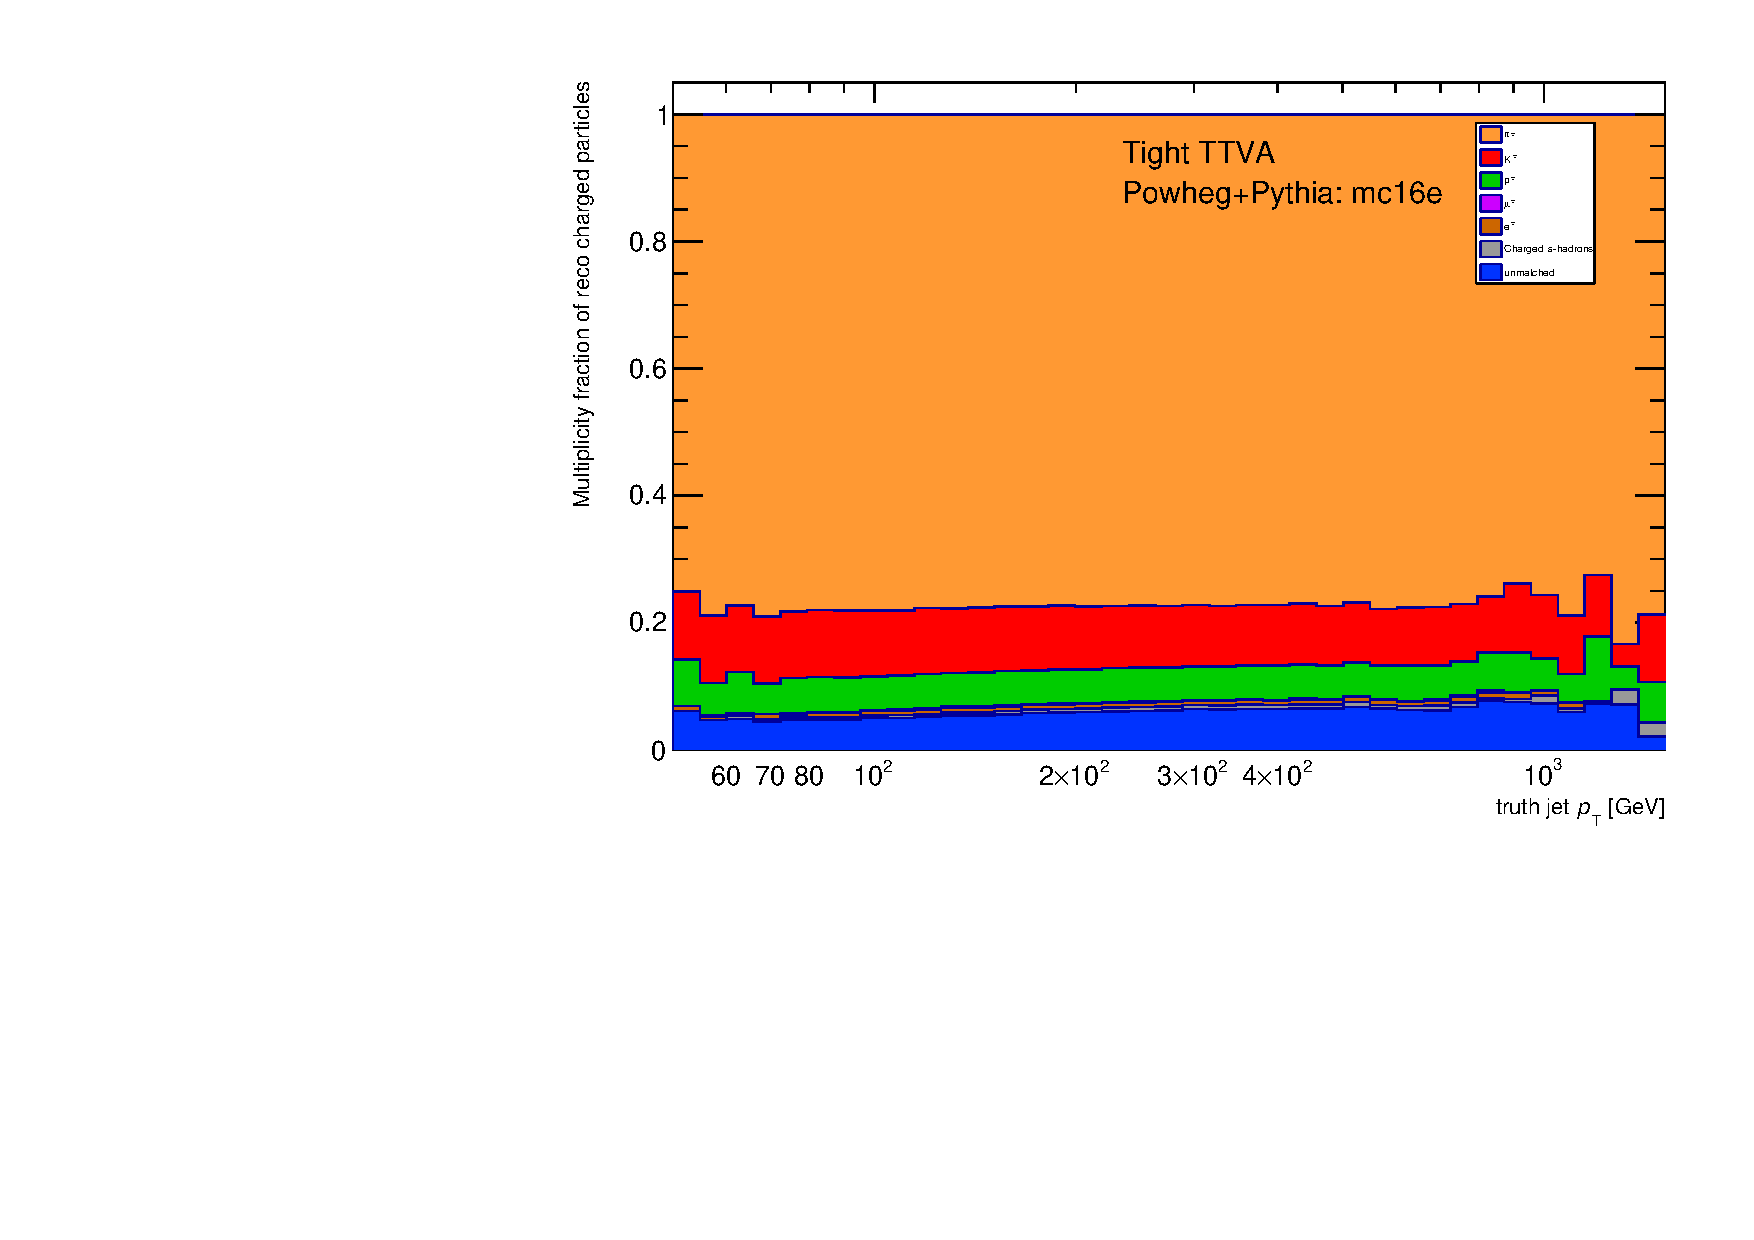
\includegraphics[width=0.48\textwidth,page=1]{figures/jetcompstudy_MultiplicityFraction.pdf}
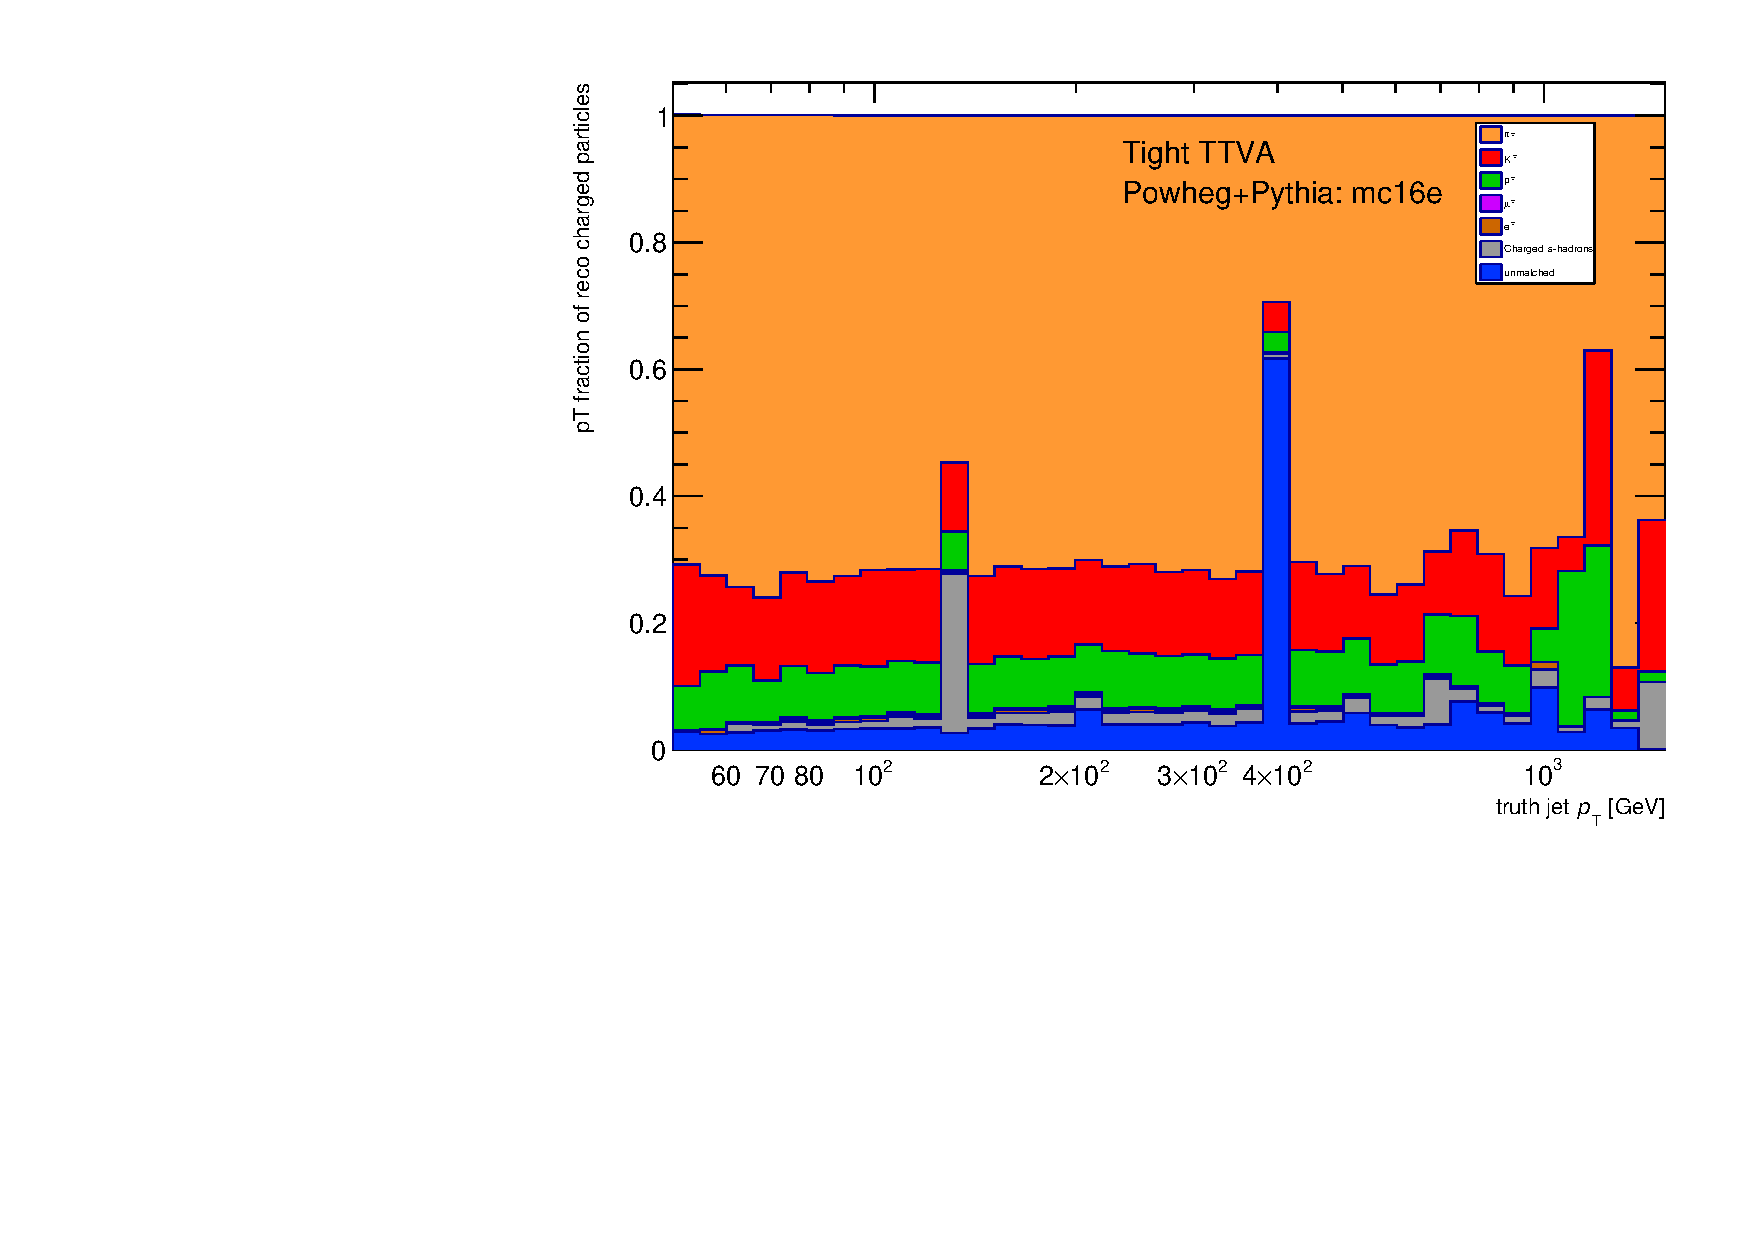
\includegraphics[width=0.48\textwidth,page=1]{figures/jet_comp_study_powheg_Tight_pTFraction_mc16e.pdf}%
\caption {The particle composition of the reconstructed tracks in terms of multiplicity (left) and \pT (right) as a function of jet \pt{}. 
This figure can be compared to Figure~\ref{fig:truthChargedJetComp} that shows the equivalent composition at particle level.}
\label{fig:trackParticleComp}
\end{figure}

Figure~\ref{fig:trackParticleComp} presents the reconstructed particle composition of tracks using the Tight TTVA working point. This figure can be compared to Figure~\ref{fig:truthChargedJetComp} that shows the equivalent plot at truth level. In case of perfect reconstruction, these plots should match.
We can see that about 7\% of Tight TTVA tracks are of the \texttt{unmatched} category, and they carry about 4\% of the \pt{}, which means that these undesired tracks have less \pt{} than the ones from the real jet constituent particles.
%We see that the reconstructed charged particle compositions indicate $\approx71$\% pions, $\approx13$\% kaons and the $\approx16$\% remaining is comprised by other charged particles.

From the composition results, we can see that charged pions are by far the dominant particle type, followed by kaons as second and protons as third.
Figure~\ref{fig:r_pion_kaon} report the track \pt{} response for pions and kaons separately for the tight and loose TTVA working point. 
Results for both these particle types are consistent: The responses for \texttt{loose} and \texttt{tight} TTVA are ~94\% and ~93\%, respectively.

\begin{figure}[tb]
\centering
\includegraphics[width=0.48\textwidth, page=4]{figures/jet_comp_study_powheg_Tight_pTFraction_mc16e.pdf}
\includegraphics[width=0.48\textwidth, page=5]{figures/jet_comp_study_powheg_Tight_pTFraction_mc16e.pdf}
\caption {The \pt{} response of pions (left) and  kaons (right) as a function of jet \pt{}, which is a proxy for the track reconstruction efficiency for these particles. 
We can see that \texttt{tight TTVA} has $\approx 93$\% tracking efficiency while \texttt{loose TTVA} improves this by $\approx 1$\%}
\label{fig:r_pion_kaon}
\end{figure}

Figure~\ref{fig:frac_unmatchedtracks} reports the \pt{} fraction of unmatched tracks separately for the \texttt{tight} and \texttt{loose} TTVA working points.
We can see that the \texttt{loose} results in about $\sim$8.4\% unmatched tracks while this is significantly reduced to $\sim$3.7\% using the tight working point.
\textbf{Since this ``fake rate'' reduction ($\approx -5$\%) is larger than the efficiency loss ($\approx -1\%$), we settle on the tight TTVA working point for the analysis}.

\begin{figure}[b]
\centering
\includegraphics[width=0.6\textwidth, page=16]{figures/jet_comp_study_powheg_Tight_pTFraction_mc16e.pdf}
\caption {The fraction of unmatched tracks w.r.t reco level jet as a function of jet \pT. We can see that \texttt{loose TTVA} has $\approx 8$\% unmatched tracks, while \texttt{tight TTVA} reduced unmatched tracks by $\approx 5$\%.}
\label{fig:frac_unmatchedtracks}
\end{figure}


%%%%%%%%%%%%%%%%%%%%
%
% 3. Closure
%


Figure~\ref{fig:r_trackjet} shows the response of all tracks associated to the reco jet. This is defined as the \pt{} of all tracks over the \pt{} of all charged particles.
This plot can be seen as a closure check from the previous two results. We see that for the tight working point, the response is about 96\%. From the previous results we would expect 93\% of the desired particles + 3.5\% from fake particles. For the loose working point, the response is 102\%, where we expect 94\% from real particles and 8\% from fakes.

\begin{figure}[tb]
\centering
\includegraphics[width=0.6\textwidth,page=17]{figures/jet_comp_study_powheg_Tight_pTFraction_mc16e.pdf}
\caption {The response of all reconstructed tracks, i.e.\ the track jet \pt{} over the charged truth jet \pt{} as a function of truth jet \pt{}. 
The \texttt{loose} TTVA shows $\approx 4$\% higher track jet response than \texttt{tight TTVA}. However \texttt{loose TTVA} introduces $\approx 5$\% more tracking inefficiencies as compare to \texttt{tight TTVA} as shown in Figure~\ref{fig:frac_unmatchedtracks}.}
\label{fig:r_trackjet}
\end{figure}


%%%%%%%%%%%%%%%%%%%%
%
% 3. Other plots
%



%, which indicates ~3\% and ~8\% unmatched tracks for \respectively. Since \texttt{tight TTVA}  selection reduces ~5\% unmatched tracks as compare to \texttt{loose TTVA}, therefore for the current analysis we are using \texttt{tight TTVA} working point.


Figure~\ref{fig:r_other} shows the \pt{} response of reconstructed tracks for protons, muons, electrons and strange hadrons.
These particles only constitute a small fraction of the jet.
The muon and electron response is lower since these particles originate from the semi-leptonic decay of heavy hadrons, so we have a (slightly) displaced production vertex.
The charged strange hadrons (which excludes kaons) are primarily $\Sigma^-$ and $\Sigma^+$, but also $\Xi^-$ and $\Omega^-$. These particles have half times $c\,\tau_0$ of 24--49~mm and decay to a neutral+charged hadron (pion or proton). So they will only give partial tracks before there is a displaced vertex (``kink'') and hence we see a lower reconstruction efficiency for these non-kaon charged strange hadrons.


\begin{figure}[tbh]
\centering
\includegraphics[scale=0.3, page=6]{figures/jet_comp_study_powheg_Tight_pTFraction_mc16e.pdf}
\includegraphics[scale=0.3, page=7]{figures/jet_comp_study_powheg_Tight_pTFraction_mc16e.pdf}
\includegraphics[scale=0.3, page=8]{figures/jet_comp_study_powheg_Tight_pTFraction_mc16e.pdf}
\includegraphics[scale=0.3, page=9]{figures/jet_comp_study_powheg_Tight_pTFraction_mc16e.pdf}
\caption {Reconstructed track response for protons (top left), muons (top right), electrons (bottom left) and charged strange hadrons (bottom right) as a function of jet \pT.}
\label{fig:r_other}
\end{figure}

%For the following composition plots \texttt{tight TTVA} selection is used to study jet composition for different particles and the comparison of individual particles fraction is shown at \texttt{reco} and \texttt{truth} level.

%Figure~\ref{fig:truthJetComp} shows the jet composition as a fraction of the particle multiplicity (left) and their momentum (right) as a function of the leading truth jet \pT{}. The $\approx 50$\% of reconstructed tracks make up pions about of the total, kaons are about $\approx 8$\% of the total and the rest $\approx 42$\% are neutral particles. The momentum fraction as a function of jet pT is shown in right in Figure~\ref{fig:truthJetComp}. The momentum fraction for different particles varies slightly as compare to multiplicity fraction.

%Figure~\ref{fig:chargedparticles} shows the fraction of the particle multiplicity (left) and their \pT{} as a function of the truth jet \pT in the particle-level jet.



%Figure~\ref{fig:chargedparticles_truthjet} shows similar plots for all the charged particles compositions in the leading jet.

%Similarly, figures~\ref{fig:pions_kaons} to ~\ref{fig:electrons_sparticles} are showing the fraction of individual particles at truth level and reconstructed level. As shown in figure~\ref{fig:chargedparticles_truthjet}, pions make most of jet fraction, and for muons, electrons and strange particles this fraction is much lower. 

% \begin{figure}[b]
% \centering
% \includegraphics[scale=0.3, page=10]{figures/jet_comp_study_powheg_Tight_pTFraction_mc16e.pdf}
% \includegraphics[scale=0.3, page=11]{figures/jet_comp_study_powheg_Tight_pTFraction_mc16e.pdf}
% \caption {The fraction of pions (left) and kaons (right) in the reconstructed tracks as a function of jet \pT, which shows  $\approx73$\% pions and $\approx14$\% kaons as reco level.}
% \label{fig:pions_kaons}
% \end{figure}

% \begin{figure}[b]
% \centering
% \includegraphics[scale=0.3, page=12]{figures/jet_comp_study_powheg_Tight_pTFraction_mc16e.pdf}
% \includegraphics[scale=0.3, page=13]{figures/jet_comp_study_powheg_Tight_pTFraction_mc16e.pdf}
% \caption {The fraction of protons (left) and muons (right) in the reconstructed tracks as a function of jet \pT, which shows  $\approx7$\% proton at reco level and fraction of muons is very low.}
% \label{fig:protons_muons}
% \end{figure}

% \begin{figure}[b]
% \centering
% \includegraphics[scale=0.3, page=14]{figures/jet_comp_study_powheg_Tight_pTFraction_mc16e.pdf}
% \includegraphics[scale=0.3, page=15]{figures/jet_comp_study_powheg_Tight_pTFraction_mc16e.pdf}
% \caption {The fraction of electrons (left) and strange particles (right) in the reconstructed tracks as a function of jet \pT.}
% \label{fig:electrons_sparticles}
% \end{figure}

\clearpage
